\documentclass[a4paper]{article}

\usepackage{a4wide}
\usepackage[utf8]{inputenc}
\usepackage[ngerman]{babel}
\usepackage{fancyhdr}
\usepackage{graphicx}
\usepackage[parfill]{parskip}
\usepackage{color}
\usepackage{enumerate}
\usepackage{url}

% fuer "deko-elemente"
\pagestyle{fancy}

% we needs moar platz
\topmargin -5mm
\headheight 73.10643pt

% include logo in document head
\chead{
\includegraphics[width=50mm]{logo.pdf}}

% seitenzahl entfernen
\cfoot{}
\rhead{}
\lhead{}

% footer content
\lfoot{\small{AlphaLabs}}
\rfoot{\small{Seite \thepage }}

% headrule
\renewcommand\headrule{
\vspace{3mm}
\footrule
}

% footrule
\renewcommand\footnoterule{\rule{\linewidth}{0pt}}

% change standard font
\usepackage[T1]{fontenc}
\newcommand{\changefont}[3]{
\fontfamily{#1} \fontseries{#2} \fontshape{#3} \selectfont}

% Tagesordnungspunkt Item
\newcommand{\TOP}[1]{\item \textbf{#1}\par}

\definecolor{dgreen}{rgb}{0.549,0.776,0.247}
\makeatletter
\def\footrule{{
  \vskip-\footruleskip\vskip-\footrulewidth
  \color{\footrulecolor}
  \hrule\@width\headwidth\@height
  \footrulewidth\vskip\footruleskip
}}
\makeatother
\renewcommand{\footrulewidth}{3pt}
\newcommand{\footrulecolor}{dgreen}

\begin{document}
\changefont{cmss}{m}{n} %computer modern sans serif

\begin{center}
\textbf{\Large The Circle of Waste - Dokumentation}
\end{center}

\vspace{5mm}


%%%%%%%%%%%%%%%%%
% HIER GEHT'S LOS
%%%%%%%%%%%%%%%%%

\tableofcontents

\pagebreak

\section{Allgemeines}
    \subsection{Inhalte und Aufbau des Lernspiels}
        Der Spieler durchläuft den ganzen Müllkreislauf, der vom Einkaufen über die Mülltrennung, Müllabfuhr und Müllverarbeitung besteht. Über das Hauptmenü kann der Spieler seinen momentanen Fortschritt sehen bzw. sehen wo im Kreislauf er sich momentan befindet und ggf. zu bereits besuchten Orten zurückspringen. An jeder der Stationen des Kreislaufs erwarten den Spieler verschiedene Aufgaben bzw. Minispiele sowie Informationen zu der speziellen Thematik.\\

    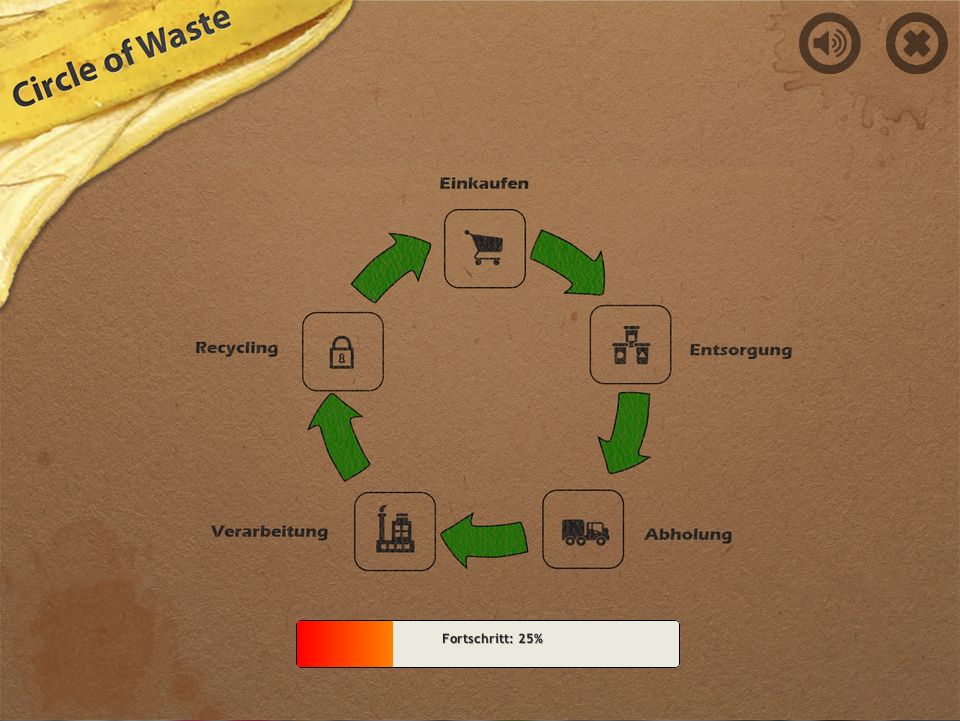
\includegraphics[width=\linewidth]{tcw.png}

    \subsection{Zielstellung}
        Das Hauptziel des Spiels ist es, den verantwortungsvollen Umgang mit Müll und der Umwelt zu vermitteln. Die Spieler sollen lernen, worauf sie beim Einkaufen von Lebensmitteln, Konsumgütern und anderen Gegenständen achten können. Welche Materialien können einfach wiederverwertet werden, welche belasten die Umwelt? Weiterhin wird dem Spieler beigebracht, welche Art von Müll wie und wo zu entsorgen ist.

\pagebreak

    \subsection{Zielgruppe}
        Das Lernspiel The Circle Of Waste richtet sich an 11-12 jährige Schulkinder, welche eine normale Schulbildung haben und lesen und schreiben können. Schulen sollen das Spiel unterrichtsbegleitend in passenden gesellschaftswissenschaftlichen Fächern nutzen können.

    \subsection{Verwendete Werkzeuge}
        Das Lernspiel \glqq The Circle of Waste\grqq\ wurde für moderne Webbrowser geschrieben und optimiert. Die dabei eingesetzten Technologien sind HTML5, CSS, und Javascript. Für die Umsetzung wurde hauptsächlich das Framework Phaser (\url{http://phaser.io/}) genutzt. Außerdem wurde an kleineren Stellen noch das Javascript Framework jQuery (\url{http://jquery.com/}) genutzt.\\
        Die Protokolle und diese Dokumentation wurden in \LaTeX\ geschrieben.\\
        Zur Versionierung und einfacherer Zusammenarbeit im Team wurde außerdem Git genutzt.\\

    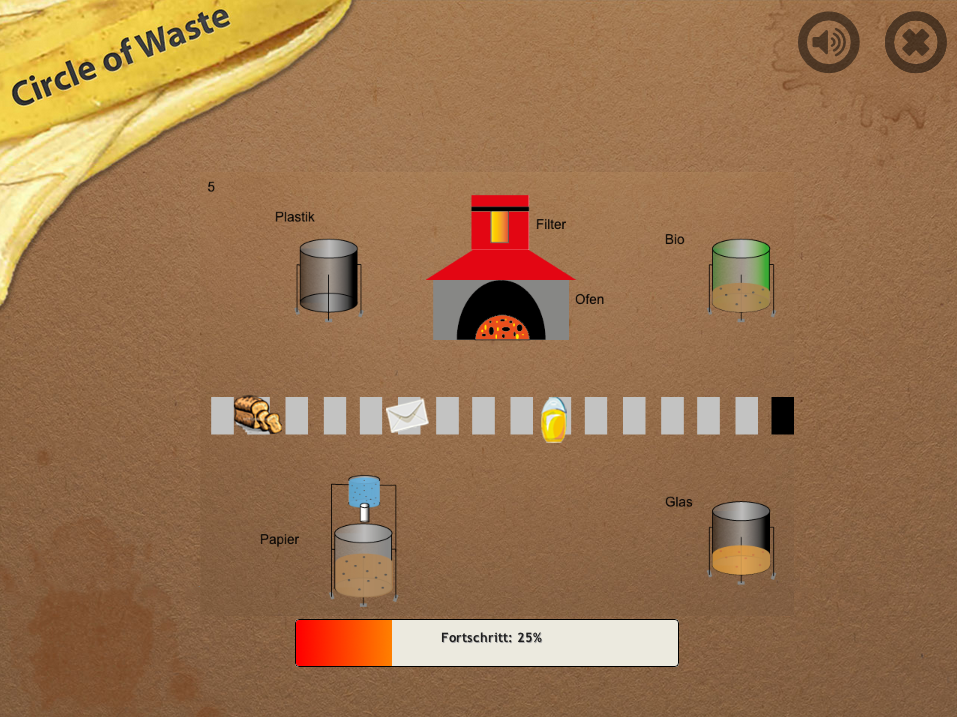
\includegraphics[width=\linewidth]{kapitel4.png}

\pagebreak

\section{Die Kapitel im Überblick}
    \subsection{Kapitel 1 - Einkaufen}
        \subsubsection{Inhalt}
            Das erste Kapitel behandelt einige Beispiele, bei denen im Alltag Müll erzeugt wird wie z.B. beim Kochen oder bei bestimmten Hobbies. Außerdem werden Charaktere vorgestellt, die im späteren Verlauf des Spiels zum Teil wieder vorkommen.
        \subsubsection{Erwartungsbild}
            Der Benutzer entwickelt ein Verständnis für den im Alltag entstehenden Müll und wie dieser verringert werden kann.
        \subsubsection{Reaktion auf Fehler}
            Fehler bei der Einschätzung von produziertem Müll werden als solche erfasst und es wird erläutert, wieso es sinnvollere Einschätzungen gibt. Zusätzlich werden Tipps zum praktischen Umgang mit diesem Müll gegeben.
        \subsubsection{Einordnung in die Lerntheorie}
            Das 1. Kapitel verknüpft verschiedene Lerntheorien, im Speziellen folgende Punkte:
            \begin{enumerate}[(a)]
                \item Behaviorismus
                \begin{enumerate}[(i)]
                    \item Lernen als Suchprozess mit Verstärkung der zufällig richtigen Reaktion\\
                    Phase 1 - Falls der Benutzer die Antwort nicht weiß hat er noch die Möglichkeit eine zufällige Antwort auszuwählen, diese wird ihm dann ggf. durch einen Applaus als richtige Antwort dargestellt.
                \end{enumerate}

                \item Kognitivismus
                \begin{enumerate}[(i)]
                    \item Lernen als vielschichtiger Prozess der Informationsverarbeitung zur Erzeugung innerer Strukturen:\\
                    Es wird in Phase 1 (Gedächtnisspiel) versucht den Benutzer dazu zu bewegen verschiedene alltägliche Tätigkeiten ins Gedächtnis zu rufen und Stück für Stück mit Charakteren aus dem Spiel zu verknüpfen. Im Folgenden wird in Phase 2 von dem Benutzer verlangt diese bereits bekannten Tätigkeiten mit ihrem Müllausstoß und Ideen zur Vermeidung in Verbindung zu bringen.\\

                    \item Wissen nicht als eingepaukte Information, sondern durch Verstehen und Verarbeiten von Informationen erwerben:\\
                    Im Phase 2 wird von dem Nutzer erwartet sich mit verschiedenen Tätigkeiten auseinanderzusetzen und diese hinsichtlich ihres Müllausstoßes zu bewerten, im Folgenden wird dem Benutzer durch weitere Informationen die Chance gegeben, seine eigenen Ideen mit gegebenen zu vergleichen.\\
                \end{enumerate}
            \end{enumerate}
            Zusammenfassend geht es in dem ersten Kapitel darum, den Nutzer langsam an das Thema Müll heranzuführen, indem zuerst gezielt bereits bekanntes Wissen abgerufen und neu verknüpft wird und im Folgenden dieses Wissen in einen Bezug zu Müll gebracht und entsprechend bewertet wird. Hierbei wird der Spieler durch Zeitliche Begrenzung motiviert und aufmerksam gehalten, sowie durch ein Punktesystem angespornt.

    \subsection{Kapitel 2 - Entsorgung}
        \subsubsection{Inhalt}
            Im 2. Kapitel wird die richtige Trennung von Müll behandelt, wozu verschiedene Müllobjekte wie z.B. Apfelreste, Bananen oder Glasflaschen, als auch Müllbehälter wie blaue Tonnen, schwarze Tonnen oder Glascontainer miteinander verknüpft werden.
        \subsubsection{Erwartungsbild}
            Der Spieler lernt auf unterhaltsame und fordernde Weise, wo er verschiedensten Müll richtig entsorgt.
        \subsubsection{Reaktion auf Fehler}
            Auftretende Fehler in Phase 1 werden gespeichert und es wird in Phase 2 explizit auf diese eingegangen um Fehlverhalten zu identifizieren und zu verbessern.
        \subsubsection{Einordnung in die Lerntheorie}
            Das 2. Kapitel verknüpft verschiedene Lerntheorien, vor allem folgende Punkte:
            \begin{enumerate}[(a)]
                \item Behaviorismus
                \begin{enumerate}[(i)]
                    \item Lernen als Konditionierungsvorgang:\\
                    In Phase 1 wird durch das Richtige Zuordnen verschiedener Müllsorten in die passenden Behälter je nach Richtigkeit positive oder negative Reize in Form von Punkten gesetzt.

                    \item Lernen als Suchprozess mit Verstärkung der zufällig richtigen Reaktion:\\
                    Falls nicht bereits im Vorfeld bekannt lernt der Spieler in Phase 1 durch Ausprobieren, ob ein Müllobjekt in einen bestimmten Behälter gehört.
                \end{enumerate}

                \item Kognitivismus
                \begin{enumerate}[(i)]
                    \item Lernen als vielschichtiger Prozess der Informationsverarbeitung zur Erzeugung innerer Strukturen:\\
                    Es werden dem Spieler in Phase 1 durch Wiederholung die Grundlagen \glqq eingehämmert\grqq\ um eine Wissensbasis zu schaffen, woraufhin in Phase 2 Informationen die zu Fehlern führten und weitere Informationen besser mit der bereits geschaffenden Basis verknüpft werden können.
                \end{enumerate}

                \item Konstruktivismus
                \begin{enumerate}[(i)]
                    \item Lernen nur durch aktive Beteiligung des Lernenden:\\
                    Der Benutzer agiert direkt mit verschiedenen Müllobjekten und Müllbehältern, indem er diese manuell verschieben und austauschen muss, wodurch er den direkten Umgang mit diesen stärker verinnerlicht.
                \end{enumerate}
            \end{enumerate}
            Zusammenfassend geht es in dem zweiten Kapitel darum, den Nutzer in der 1. Phase durch Wiederholung der selbst zuzuordnenden Gegenstände und direkter Resonanz, die richtige Trennung von Müll zu „erkunden“zu lassen. Im Folgenden werden in Phase 2 Quellen die zu Fehlverhalten geführt haben behandelt und Missverständnisse aus dem Weg geräumt.

    \subsection{Kapitel 3 - Abholung}
        \subsubsection{Inhalt}
            Im Kapitel 3 wird die Abholung des produzierten Mülls behandelt. Dazu werden die verschieden Mülltonnen mit den verschiedenen Müllsorten von verschiedenen Müllwagen abgeholt.
        \subsubsection{Erwartungsbild}
            Der Benutzer erhält Grundkenntnisse über den Prozess der Müllabholung und sollte in der Lage sein den Müll zu unterscheiden.
        \subsubsection{Reaktion auf Fehler}
            Bei falscher Müllabholung werden im Spiel Punkte abgezogen, sollten diese unter 0 gehen geht ein Leben verloren. Bei 0 Leben ist das Spiel vorbei; ebenso, wenn man in den Abgrund fällt.
        \subsubsection{Einordnung in die Lerntheorie}
            Das 3. Kapitel verknüpft verschiedene Lerntheorien, im Speziellen folgende Punkte:
            \begin{enumerate}[(a)]
                \item Behaviorismus
                \begin{enumerate}[(i)]
                    \item Lernen der Müllabholung durch Informationen dazu.
                \end{enumerate}

                \item Kognitivismus
                \begin{enumerate}[(i)]
                    \item Lernen als Prozess der Erkenntnis das Müllabholung und Mülltrennung eng beieinander liegen. Erkenntnis durch spezielle Fahrzeugfarben, die nur entsprechende Tonnen einsammeln, zugleich werden Hinderniss aufgestellt die überwunden werden müssen.
                \end{enumerate}
            \end{enumerate}

    \subsection{Kapitel 4 - Verarbeitung}
        \subsubsection{Inhalt}
            Im 4. Kapitel geht das Lernspiel auf die Verarbeitung der verschieden Müllsorten ein. Es wird eine virtuelle Müllverarbeitungsanlage dargestellt, in der ein Förderband konstant neuen Müll anliefert und der Spieler den Müll in die verschiedenen Stationen einsortieren muss. Zusätzlich zum sortieren des Mülls, müssen die Stationen bedient werden. Z.B. muss der Verbrennungsofen geleert werden und der Smog gefiltert werden.
        \subsubsection{Erwartungsbild}
            Der Spieler bekommt eine Vorstellung von Müllverarbeitungsanlagen und lernt auf spielerische Art und Weise, wie die verschiedenen Müllsorten verarbeitet werden. Welcher Müll wird direkt verbrannt, welcher wird anderweitig verarbeitet?
        \subsubsection{Reaktion auf Fehler}
            Sollte der Spieler eine Müllelement falsch zuordnen, wird es nicht von der jeweiligen Station angenommen und zurück auf das Förderband gelegt. Der Spieler hat nochmals die Chance sich zu verbessern, allerdings bleibt ihm dafür weniger Zeit und der nächste Müll wartet schon.
        \subsubsection{Einordnung in die Lerntheorie}
            Das 4. Kapitel verknüpft verschiedene Lerntheorien, vor allem folgende Punkte:
            \begin{enumerate}[(a)]
                \item Behaviorismus
                \begin{enumerate}[(i)]
                    \item Es werden durch das Zuordnen der verschiedenen Müllsorten positive oder negative Reize in Form von Punkten gesetzt.

                    \item Lernen als Suchprozess mit Verstärkung der zufällig richtigen Reaktion:\\
                    Falls nicht bereits im Vorfeld bekannt lernt der Spieler durch Ausprobieren, ob ein Müllelement in die richtige Station eingeordnet wurde.
                \end{enumerate}
            \end{enumerate}

\section{Evaluation}
    \subsection{Erreichen der Ziele}
        Es wurde ein vollständig benutzbares Spiel entwickelt, welches einige Lernaspekte übermitteln kann. Allerdings gab es auch einige Ziele, die wir nicht erreichen konnten:
        \begin{enumerate}[(a)]
            \item Das komplette Kapitel 5 wurde leider nicht fertiggestellt
            \item Die anderen Kapitel haben noch Verbesserungsbedarf in verschieden Hinsichten (meistens Kleinigkeiten, die wir uns anders vorgestellt haben)
            \item Aufgrund mangelnder Kentnisse und Kreativität ist das Design des Lernspiels nicht wie ursprünglich vorgestellt
            \item HTML5 bzw. Phaser war ein interessantes Entwicklungswerkzeug und wir haben dabei auch nützliche Dinge gelernt (im Gegensatz zu einer fast \glqq toten\grqq\ Technologie wie z.B. Flash). Allerdings war die Entwicklung deswegen wohl etwas schwieriger und zeitintensiver
        \end{enumerate}
        Zusammenfassend müssen wir sagen, dass ein paar Ziele leider aufgrund von Zeitmangel (siehe Zeitplanvergleich) nicht erreicht wurden.

    \pagebreak

    \subsection{Zeitplanvergleich}
        Der ursprünglich erstelle Zeitplan stellte die einzelnen (Teil-)Abgaben sowie unsere Arbeitspakete dar:\\\\
        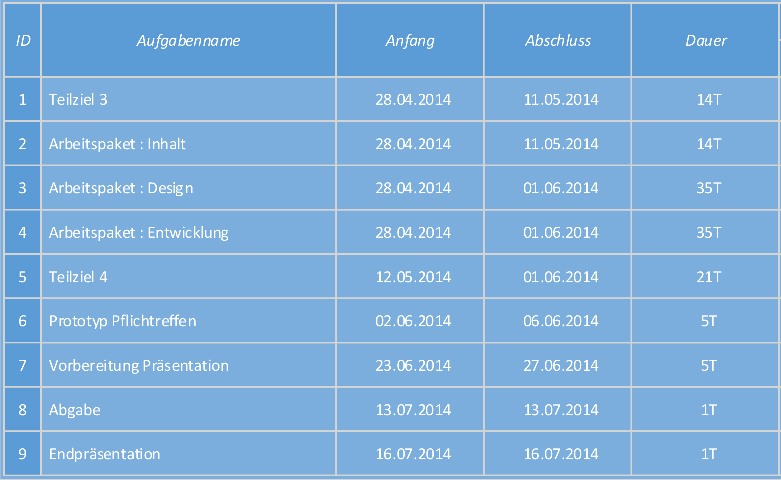
\includegraphics[width=\linewidth]{zeitplan_1}\\\\
        Im Rückblick war der Zeitplan zu locker erstellt und die Zeiträume waren falsch gesetzt. Wir konnten allerdings alle Teilziele rechtzeitig und zufriedenstellend abgeben. Die Arbeitspakete konnten bis einige Tage vor der Abgabe nicht fertig gestellt werden, da immer wieder an Inhalten, Design (hauptsächlich Bilder) und dem Programmcode gearbeitet werden musste. Auch die Erstellung der Präsentation musste so gezwungendermaßen nach hinten verschoben werden.\\
        Es wäre besser gewesen, die einzelnen Arbeitspakete noch weiter zu unterteilen (z.B. auch auf die Kapitel) um den Fortschritt besser zu sehen.\\
        \\
        Zusammenfassend war am Ende des Semesters vor der Abgabe noch einiges zu tun, weswegen auch einige Sachen auf der Strecke geblieben sind und Verbesserungen nicht eingebaut wurden.

%%%%%%%%%%%%%%%%%%%
% HIER IST'S VORBEI
%%%%%%%%%%%%%%%%%%%

\end{document}
